\subsection{Surrogate Performance and Relevant Dimensions}

The reduced Gaussian-process (GP) surrogates approximate the UCED mismatch surface on observations excluded from model development (Fig.~\ref{fig:gp_holdout_validation}). Five-fold pooled cross-validated $R^2$ values on the development sets are 0.9988 for 2016 and 0.9853 for 2021. On the independent held-out UCED evaluations, the corresponding $R^2$ values are 0.9987 and 0.9933, with root-mean-square errors of $1.08\times10^{-4}$ and $1.42\times10^{-4}$, respectively, on the original $L(\theta)$ scale ($n=20$ for each year). The held-out Spearman correlations are 1.000 and 0.992. These diagnostics support using the reduced GPs for subsequent offline exploration together with direct UCED revalidation of selected region members; they do not establish parameter recoverability.

The fixed-kernel, five-fold ARD screen excludes a dimension when its fitted length scale reaches the prescribed upper bound in at least four folds. For 2016, this rule retains three dimensions: the physical MLT contract band and the non-retrofitted CHP minimum-output parameters for the 300--660 MW and 0--300 MW classes. For 2021, it retains those same three dimensions together with the retrofitted-coal minimum-output parameters for the 300--660 MW and 0--300 MW classes and the retrofitted-coal minimum up/down-time parameter for the 0--300 MW class. All three 2016 retained dimensions remain below the bound in all five folds. In 2021, four retained dimensions remain below it in all five folds; the 0--300 MW retrofitted-coal minimum-output and minimum up/down-time dimensions reach the bound in three and two folds, respectively, and are retained under the four-of-five rule. The fold-level screen is shown in Fig.~\ref{fig:supp_ard_fold_stability}. These ARD results identify dimensions retained for surrogate construction, not parameter estimates, causal effects, or a ranking of physical importance.

Using exactly the same held-out observations for the full and reduced fits, the 2016 test $R^2$ changes from 0.9979 to 0.9987 ($\Delta R^2=+0.0008$), while RMSE decreases from $1.39\times10^{-4}$ to $1.08\times10^{-4}$. For 2021, test $R^2$ changes from 0.9936 to 0.9933 ($\Delta R^2=-0.0003$), and RMSE increases from $1.39\times10^{-4}$ to $1.42\times10^{-4}$. The corresponding pooled development-set cross-validated $R^2$ values increase from 0.9982 to 0.9988 in 2016 and from 0.9790 to 0.9853 in 2021. The reduced surrogates therefore preserve held-out predictive performance while providing lower-dimensional representations. Additional ARD checks retain the 2021 baseline set across the tested length-scale ceilings; the 2016 set is ceiling-sensitive because one excluded duration dimension becomes retained at the doubled ceiling. Cross-fitted reduced models improve RMSE in both years. Full results are reported in the Supplementary Material.

\begin{figure*}[t]
\centering
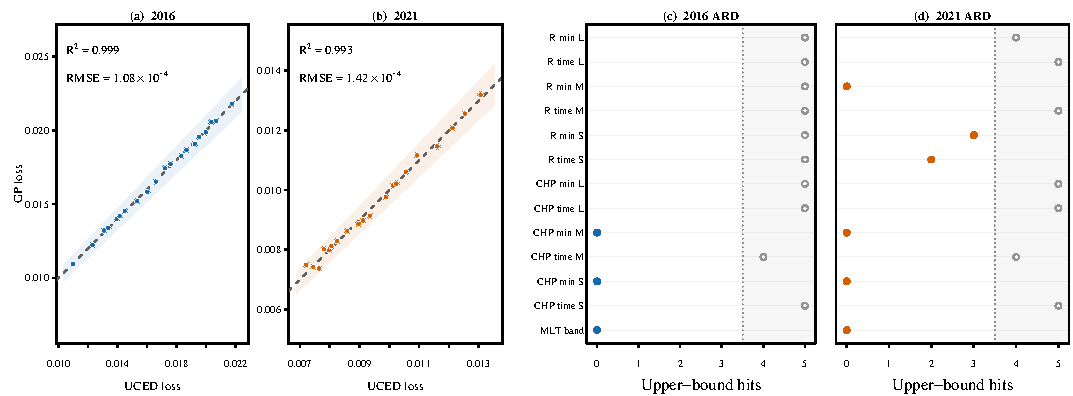
\includegraphics[width=\textwidth]{fig_surrogate_performance_active_parameters_ieee.pdf}
\caption{Held-out surrogate validation and retained parameter dimensions. Panels (a) and (b) compare the mismatch obtained from an original UCED evaluation with the corresponding reduced-GP prediction for observations excluded from model development; dashed lines denote perfect agreement and shaded bands denote $\pm5\%$. Panels (c) and (d) summarize the fold-wise ARD screen. Filled markers denote retained dimensions, open markers denote excluded dimensions, and the shaded area marks the four-or-five upper-bound hits that trigger exclusion. R and CHP denote retrofitted coal and non-retrofitted CHP; L, M, and S denote the 660--1000, 300--660, and 0--300 MW classes.}
\label{fig:gp_holdout_validation}
\end{figure*}

% Supplementary figure:
% 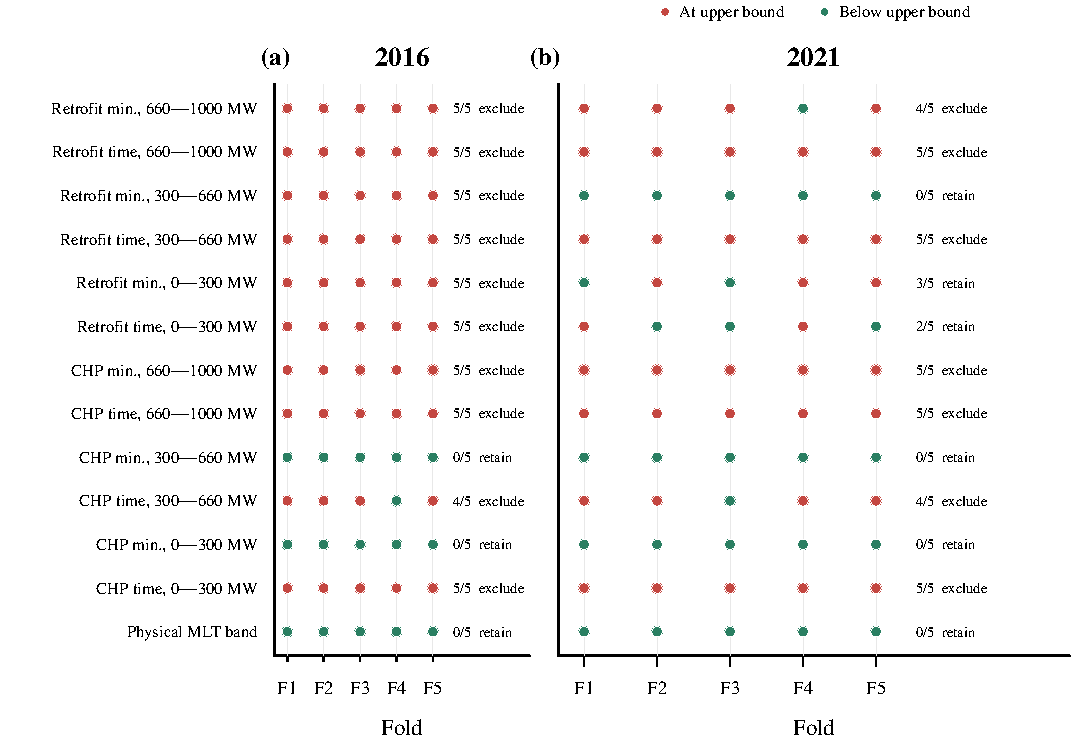
\includegraphics[width=\textwidth]{supp_ard_fold_stability.pdf}
% \caption{Fold-wise stability of ARD screening. Red markers indicate that the fitted
% length scale reached the prescribed upper bound in that fold; green markers indicate
% a value below the bound. A parameter is excluded after at least four upper-bound hits.}
% \label{fig:supp_ard_fold_stability}
